\section{Sito}
Il sito è raggiungibile all'url \href{http://tassinari.info:8080}{tassinari.info:8080} gira su un container docker su un raspberry pi 4.\\
Per il testing è possibile creare un account o accedere ad uno già fatto con username e password "user" "user".\\
I sorgenti sono disponibili su github: \href{https://github.com/leo-tasso/Hilfe}{github.com/leo-tasso/Hilfe}\\
Per qualsiasi dubbio o richiesta è possibile contattarci \href{mailto:leonardo.tassinari6@studio.unibo.it}{leonardo.tassinari6@studio.unibo.it}
\section{Mission}
Il sito è un social network scritto in PHP per coordinare, gestire e supportare l'aiuto volontario sociale. Il nome deriva dal verbo "aiutare" in tedesco che compone l'acronimo: "Hands in love fostering empowerment".
L'idea è nata dalle alluvioni che hanno colpito la Romagna nel 2023; in quel momento, l'uso di una piattaforma del genere sarebbe potuto essere di grande aiuto per la gestione del supporto alla popolazione colpita e per i potenziali volontari.
\section{Brand Identity}
Il logo e il design del sito sono semplici, diretti, leggeri e gradevoli in modo da aggevolare l'esperienza utente e di facilitare l'utilizzo della piattaforma.
I colori scelti per il logo sono \textcolor[HTML]{087E8B}{\#087E8B} e \textcolor[HTML]{BB0112}{\#BB0112}.\\
Il primo secondo la psicologia dei colori suggerisce potenza e sicurezza mentre il rosso richiama l'amore e la passione, tutti temi affini alla mission.
\section{Sviluppo}
Per lo sviluppo ci siamo avvalsi di diversi focus group con utenti target di età variabile, in modo da comprendere i casi d'uso e migliorare l'usabilità.
\begin{figure}[H]
    \centering
    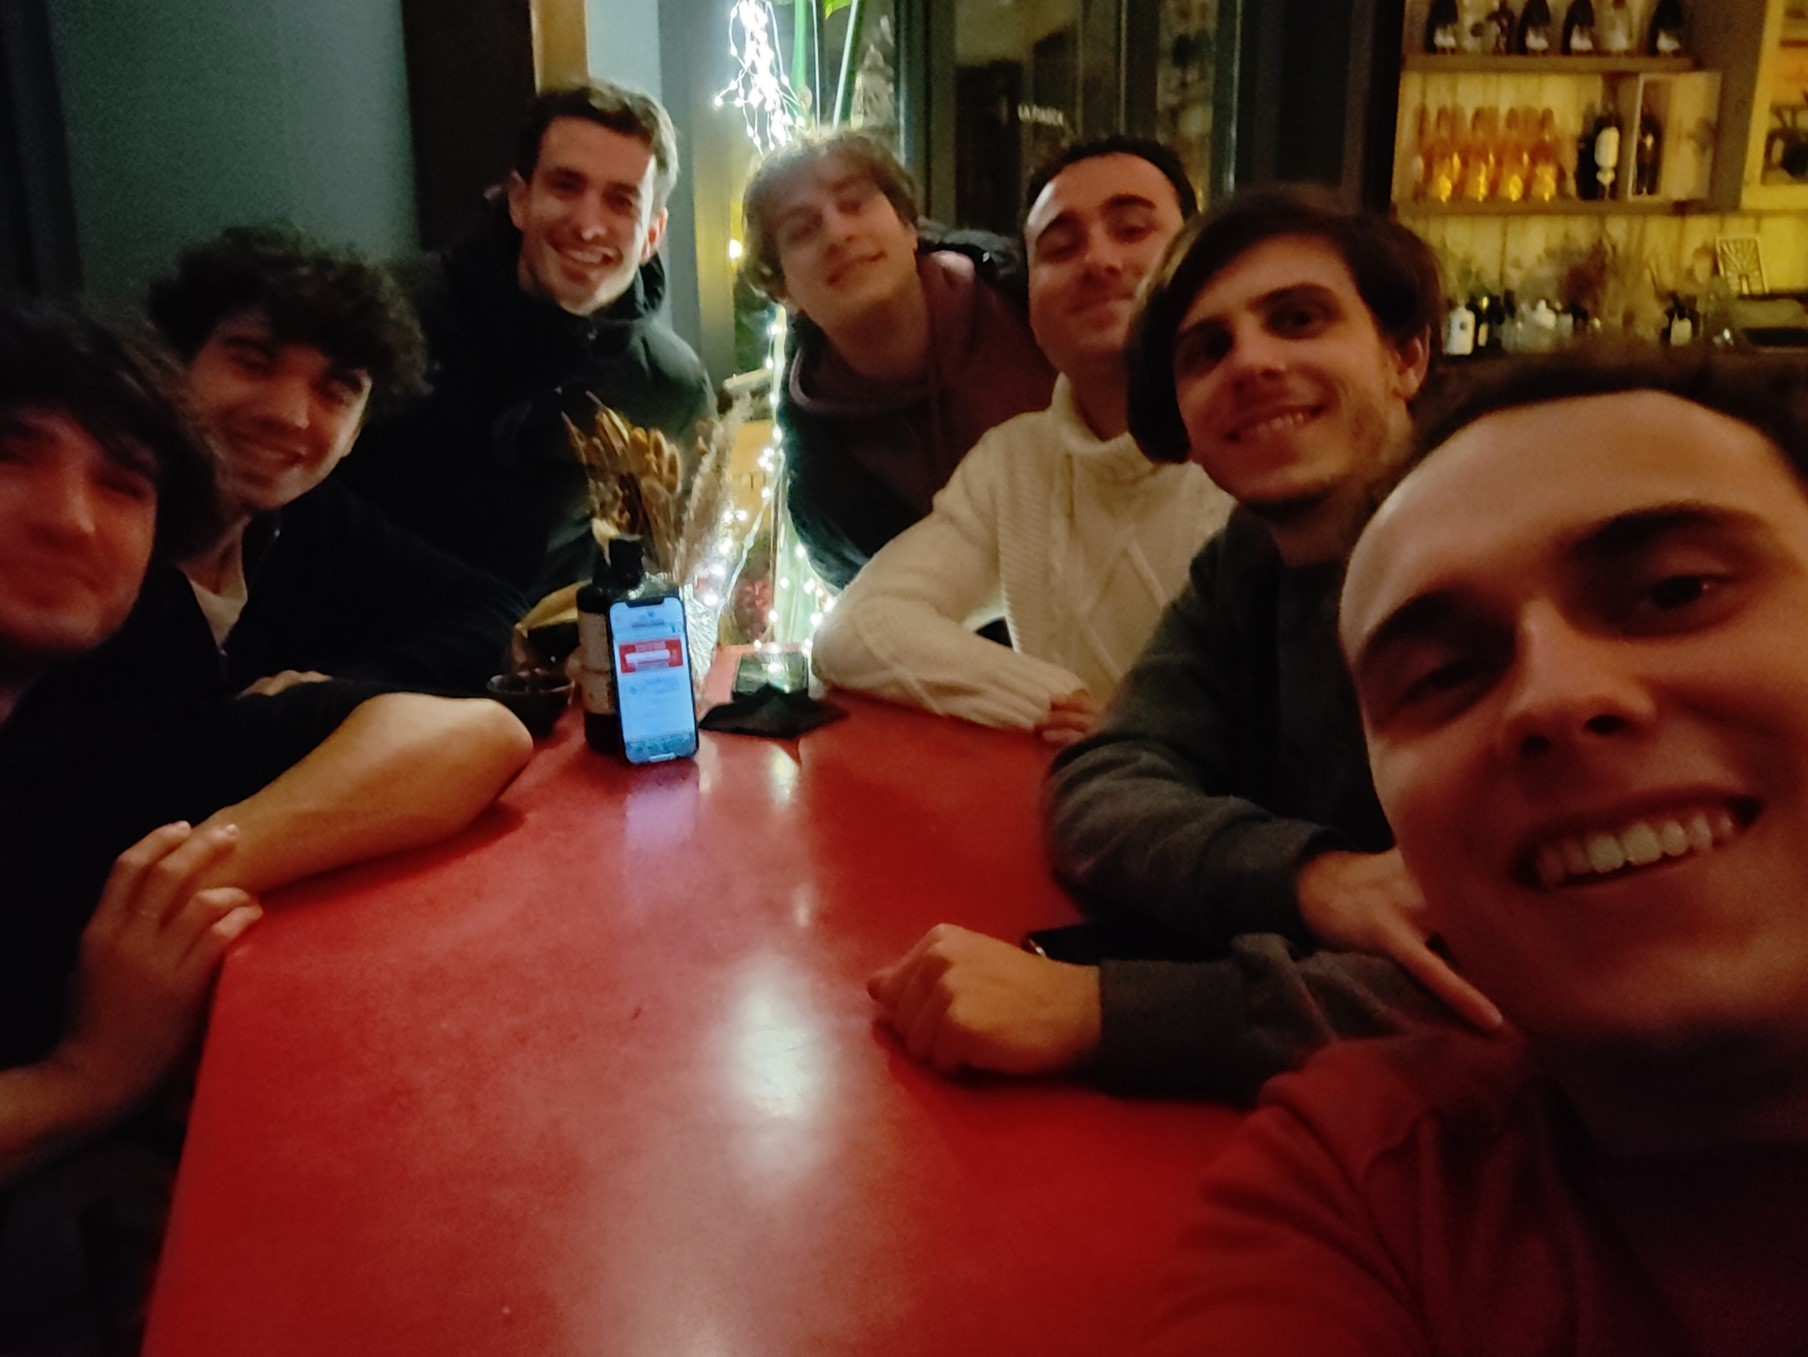
\includegraphics[width=0.5\textwidth]{focusGroup.jpg}
\end{figure}
\section{Accessibilità}
Per la verifica dell'Accessibilità abbiamo controllato le pagine principali su:\\
\href{https://validator.w3.org/}{https://validator.w3.org/} Per verificare di avere codice valido.\\
\href{https://achecks.org/achecker/}{https://achecks.org/achecker/} Per verificare di avere codice il più accessibile possibile.\\
\href{https://webaim.org/resources/contrastchecker/}{https://webaim.org/resources/contrastchecker/} Per verificare che tutte le combinazioni di colori scelte avessero un contrasto adeguato anche per utenti ipovedenti.
\section{Autori}
\begin{minipage}[t]{0.4\textwidth}
    \textbf{Leonardo} \textbf{Tassinari}\\
    \href{mailto:leonardo.tassinari6@studio.unibo.it}{leonardo.tassinari6@studio.unibo.it}
\end{minipage}%
\hfill
\begin{minipage}[t]{0.3\textwidth}
    \begin{tikzpicture}
        \node[draw=blue, circle, inner sep=35pt, path picture={\node at (path picture bounding box.center){
\includegraphics[width=4cm]{leo.jpg}};}] at (0,0) {};
    \end{tikzpicture}
\end{minipage}
\begin{minipage}[t]{0.4\textwidth}
    \textbf{Alessandra} \textbf{Versari}\\
    \href{mailto:alessandra.versari2@studio.unibo.it}{alessandra.versari2@studio.unibo.it}
\end{minipage}%
\hfill
\begin{minipage}[t]{0.3\textwidth}
    \begin{tikzpicture}
        \node[draw=blue, circle, inner sep=35pt, path picture={\node at (path picture bounding box.center){
\includegraphics[width=5cm]{sandra.jpg}};}] at (0,0) {};
    \end{tikzpicture}
\end{minipage}